\documentclass{article}
\usepackage[utf8]{inputenc}

\title{Basic Of Deep Learning - Mid Semester Project Part 1}
\author{Guy Houri, Yoav Gal}
\date{Submitted as mid-semester project report for Basic Of Deep Learning course, Colman, 2024}

\usepackage{natbib}
\usepackage{graphicx}
\usepackage{algpseudocode}
\usepackage{algorithm}
\usepackage{amsmath}
\usepackage{color}
\usepackage{tcolorbox}
\usepackage{hyperref} 
\usepackage{amsmath}
\usepackage{listings}
\usepackage{url}

\lstset{
    language=Python,
    basicstyle=\ttfamily\footnotesize,
    numbers=left,
    breaklines=true,
    frame=single,
    captionpos=b, % Caption below the listing
    tabsize=4
}

\begin{document}

\maketitle

\section{Introduction}

Image classification has emerged as a cornerstone of modern computer vision, enabling machines to recognize and categorize visual information with remarkable accuracy. This project delves into the realm of binary image classification, specifically focusing on distinguishing between images of fingers displaying the digits "0" and "5." \\

This project leverages core deep learning techniques to address the image classification task. The use of a neural network with a hidden layer allows the model to learn complex nonlinear relationships between input pixels and class labels. Backpropagation, a fundamental algorithm in deep learning, enables the network to iteratively refine its parameters by propagating the error signal back through the network and adjusting the weights accordingly. The choice of the sigmoid activation function and the cross-entropy loss function are crucial for binary classification problems, facilitating efficient training and accurate predictions. By employing these deep learning techniques, the model can effectively extract meaningful features from the input images and achieve high classification accuracy. \\

Through this project, our aim is to:
1.  Develop a functional image classification model for the given task.
2.  Investigate the impact of different hyperparameters on model performance.
3. Gain practical experience in the implementation and training of a neural network.
4.  Deepen our understanding of the core concepts and techniques in deep learning. \\

This report will detail the data preprocessing steps, model architecture, training process, and evaluation results. In addition, we will discuss the challenges encountered during the project and potential avenues for future improvement. 


\subsection{Data}
The data set we will be working on is called Sign Language Digits. This data set contains 5,000 black and white images divided into 10 different types of hand sign representing numbers 0 to 9. The size of each individual image is 28x28 pixels. The data set file is a NumPy array containing the image pixels. It includes 5,000 rows for each image and 784 columns for each pixel in the image (28x28).


\subsection{Problem}
This project tackles the challenge of recognizing handwritten digits in sign language from images. Sign language presents unique challenges for image classification due to the inherent variability in human hand gestures. Factors such as differences in hand size, orientation, lighting conditions, and individual variations in hand shape can significantly impact the accuracy of digit recognition.

\section{Solution}
\subsection{General approach}
This project employs a supervised machine learning approach. A feedforward neural network with a single hidden layer is utilized to classify the images. The network processes the raw pixel data from each image and learns to extract relevant features through the hidden layer. The output layer generates a probability for each class (0,5). This architecture allows the model to learn complex nonlinear relationships between the input pixels and the corresponding digit.

\subsection{Design}

\subsubsection{Environment}
This project was implemented and executed using a Jupyter Notebook environment hosted on Google Colaboratory (Colab). The notebook, saved in the .ipynb format, provided an interactive platform for code development, experimentation, and documentation. Python, with its extensive collection of libraries specifically designed for numerical computation (NumPy), machine learning (scikit-learn), was used throughout the project. Colab's cloud-based infrastructure offered access to necessary computational resources and we were able to run our model in a very short time.

\subsubsection{Architecture}
\underline{Pre Processing} \\ 
Filter, Normalize, and Split to train and test.
\begin{lstlisting}
# filter
mask = (y == "0") | (y == "5")
X_filtered = X[mask]
Y_filtered = y[mask]

# Normalize
X = X_filtered/255.0 # to become value from 0-1 insted of 0-255

# Split
indices = np.random.permutation(X.shape[1]) 
split_point = int(0.8 * X.shape[1])
X_train, X_test = X[:, indices[:split_point]], X[:, indices[split_point:]]
Y_train, Y_test= Y[:, indices[:split_point]], Y[:, indices[split_point:]]
\end{lstlisting} 

\underline{Activation function} \\
We chose sigmoid. This introduces curves and bends, allowing the network to learn more complex patterns and relationships in the data through non linear transformations.
\begin{lstlisting}
def sigmoid(x):
    return 1 / (1 + np.exp(-x))
\end{lstlisting}

\underline{Loss function} \\
Binary cross-entropy - measures the dissimilarity between predicted probabilities and true binary labels (0 or 1), quantifying the error of a binary classification model's predictions. in the function we avoid log(0) by assigning y-hat a value that is closeToZero with numpy clip function
\begin{lstlisting}
def log_loss(y_hat, y):
    closeToZero = 1e-15
    y_hat = np.clip(y_hat, closeToZero, 1 - closeToZero)
    loss = - (y * np.log(y_hat) + (1 - y) * np.log(1 - y_hat))
    return loss
\end{lstlisting}

\underline{Hyperparameters} \\
Hyperparameters are settings that are set before training a machine learning model and control the learning process itself, influencing how the model learns the underlying patterns in the data. Our input layer is 784 features (28*28) pixels. \\
\textbf{Hidden layer} - we chose a hidden layer of 128 neurons. A larger hidden layer can potentially learn more complex patterns, but also increases the risk of overfitting (memorizing the training data instead of generalizing to new data). A smaller hidden layer might not have enough capacity to learn the underlying patterns. In our case, 128 worked well. In computer science, powers of 2 are often preferred for memory allocation and data processing because they align well with the binary nature of computers. \\
\textbf{Learning rate} - During training, the neural network adjusts its weights and biases to minimize the loss function. The learning rate scales the gradient of the loss function, determining how much weights and biases are updated in each iteration. In our case, we chose 0.01 \\
\textbf{Epochs} - the number of times the entire training dataset is passed through the neural network during training. More epochs allow the model to learn more from the data, but too many epochs can lead to overfitting. for our case epochs=100 was fine. \\
\textbf{Batch Size} - controls how many training examples are processed in each iteration of the training process. It affects the stability of the gradients, memory usage, and training speed. our batch size is 32. \\

\underline{Forward Propagation} \\
Multiplying neurons by weights and adding biases, after which they are passed through the activation function.
\begin{lstlisting}
Z1 = np.matmul(W1, X_batch) + b1
A1 = sigmoid(Z1)  # Store sigmoid output for reuse
Z2 = np.matmul(W2, A1) + b2
A2 = sigmoid(Z2)
\end{lstlisting} 

\subsubsection{Back Propagation}
Back Propagation is the calculations of gradients of the loss function with respect to the network's weights. These gradients are then used to update the weights, iteratively minimizing the error and improving the network's performance. The gradients indicate the direction of the steepest ascent of the loss function. Backpropagation calculates the negative of the gradients to find the direction of steepest descent (towards the minimum). We calculate the gradient by the derivative.

\begin{algorithm}
\caption{Gradient Descent}
\label{alg:gradient_descent}
\begin{algorithmic}[1] % Numbered lines

\Require Training data $(X, Y)$, Loss function $L(\theta)$, Learning rate $\eta$, Initial parameters $\theta$

\Ensure Optimized parameters $\theta$

\While{not converged or maximum iterations reached}
    \State $\nabla L(\theta) \gets \text{Calculate gradient of } L(\theta) \text{ with respect to } \theta$ \Comment{Compute the gradient}
    \State $\theta \gets \theta - \eta \cdot \nabla L(\theta)$ \Comment{Update parameters}
\EndWhile

\State \textbf{return} $\theta$

\end{algorithmic}
\end{algorithm}

\textbf{Derivative Calculation} \\
\textbf{${dZ_2}$ = $\frac{dL}{dZ_2}$  = $\frac{dL}{dA_2}$ * $\frac{dA_2}{dZ_2}$} (chain rule) \\
we begin the backward pass by considering the derivative of the loss function L. oss L is not directly a function of Z2. It's a function of A2, which is a function of Z2. We need the chain rule to "bridge the gap."
\begin{align}
\frac{dL}{da} &= \frac{d}{da} \left( -[y \cdot \log(a) + (1-y) \cdot \log(1-a)] \right) \\
&= -\left[ y \cdot \frac{1}{a} - (1-y) \cdot \frac{1}{1-a} \right] \\
&= -\frac{y}{a} + \frac{1-y}{1-a} \\
&= \frac{-y(1-a) + (1-y)a}{a(1-a)} \\
&= \frac{-y + ay + a - ay}{a(1-a)} \\
&= \frac{a - y}{a(1-a)}
\end{align}

Therefore:

\begin{equation}
\frac{dL}{dA_2} = \frac{A_2 - y}{A_2(1-A_2)}
\end{equation}

To find the derivative $\frac{dA_2}{dZ_2}$, we can rewrite the sigmoid function as:

\begin{equation}
A_2 = (1 + e^{-Z_2})^{-1}
\end{equation}

\begin{align}
\frac{dA_2}{dZ_2} &= \frac{e^{-Z_2}}{(1 + {e^{-Z_2}})^2} \\
&= \frac{1}{1 + e^{-Z_2}} \cdot \frac{e^{-Z_2}}{1 + e^{-Z_2}} \\
&= \frac{1}{1 + e^{-Z_2}} \cdot \left(1 - \frac{1}{1 + e^{-Z_2}}\right) \\
&= A_2 \cdot (1 - A_2)
\end{align}

Therefore:

\begin{equation}
\frac{dA_2}{dZ_2} = A_2(1 - A_2)
\end{equation}


\begin{align}
\frac{dL}{dZ_2} &= \frac{dL}{dA_2} \cdot \frac{dA_2}{dZ_2} \\
&= \frac{A_2 - y}{A_2(1-A_2)} \cdot A_2(1-A_2) \\
&= A_2 - y
\end{align}

This is why, in many implementations with sigmoid output and binary cross entropy, you directly see $\frac{dL}{dZ_2} = A_2 - y$ being used in the backpropagation calculations.
\begin{lstlisting}
dZ2 = (A2 - Y_batch.reshape(1, -1))
\end{lstlisting}

\textbf{dW2}

\begin{equation}
Z_2 = W_2 A_1 + b_2
\end{equation}

\begin{equation}
\frac{\partial L}{\partial W_2} = \frac{\partial L}{\partial Z_2} \frac{\partial Z_2}{\partial W_2}
\end{equation}

Thus:
\begin{equation}
\frac{\partial Z_2}{\partial W_2} = A_1
\end{equation}

\begin{equation}
\frac{\partial L}{\partial W_2} = \frac{\partial L}{\partial Z_2} A_1
\end{equation}

\begin{lstlisting}
dW2 = np.matmul(dZ2, A1.T) / batch_size 
\end{lstlisting}

\textbf{dB2}
\begin{equation}
\frac{\partial L}{\partial B_2} = \frac{\partial L}{\partial Z_2} \frac{\partial Z_2}{\partial B_2}
\end{equation}

Thus:
\begin{equation}
\frac{\partial Z_2}{\partial B_2} = 1
\end{equation}

\begin{equation}
\frac{\partial L}{\partial B_2} = \frac{\partial L}{\partial Z_2}
\end{equation}

\begin{lstlisting}
db2 = np.sum(dZ2, axis=1, keepdims=True) / batch_size
\end{lstlisting}

All the code Together:
\begin{lstlisting}
dZ2 = (A2 - Y_batch.reshape(1, -1)) # Reshape Y_batch for proper subtraction
dW2 = np.matmul(dZ2, A1.T) / batch_size # Average over batch
db2 = np.sum(dZ2, axis=1, keepdims=True) / batch_size # Average over batch

dA1 = np.matmul(W2.T, dZ2)
dZ1 = np.multiply(dA1, sigmoid_derivative(Z1)) # Reuse sigmoid output (A1)
dW1 = np.matmul(dZ1, X_batch.T) / batch_size # Average over batch
db1 = np.sum(dZ1, axis=1, keepdims=True) / batch_size # Average over batch

# Update weights
W2 = W2 - learning_rate * dW2
b2 = b2 - learning_rate * db2
W1 = W1 - learning_rate * dW1
b1 = b1 - learning_rate * db1\end{lstlisting} 

\section{Base Model}

Our model recives a 28*28 pixel matrix, where each value is between 0-255. afterwards we process the data to be between 0-1. the matrix represents a grayscale image of a sign symbol 0 or 5. The output of the model is a number between 0-1, the closer it is to 0 - the model guesses that the sign is 0. the closer it is to 1 - the model guesses that the sign is 5. \\
Prediction Examples:
\begin{figure}[H]
    \begin{minipage}[b]{0.45\textwidth} % Adjust 0.48 for spacing
        \centering
        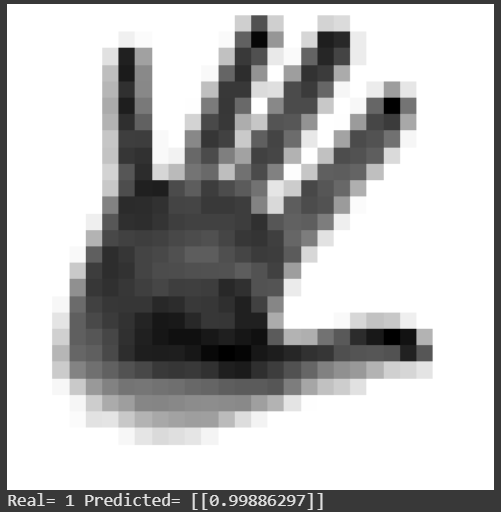
\includegraphics[width=\textwidth]{figures/predictedOne.png}
        \caption{Predicted sign 5}
        \label{fig:predictedOne}
    \end{minipage}
    \hfill % Horizontal space between the minipages
    \begin{minipage}[b]{0.45\textwidth} % Adjust 0.48 for spacing
        \centering
        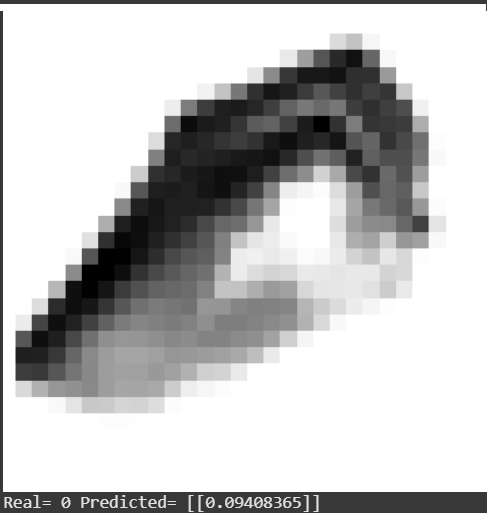
\includegraphics[width=\textwidth]{figures/predictedZero.png}
        \caption{predicted sign 0}
        \label{fig:predictedZero}
    \end{minipage}
\end{figure}


\subsection{Results and Metrics}

This section presents the results of the trained neural network model on the sign language digit classification task. The model's performance is evaluated using various metrics, including loss, accuracy, precision, recall, and the confusion matrix. \\

\subsubsection{Loss}
The training process was monitored by tracking the binary cross-entropy loss function. As shown in Figure 1, the training loss decreased steadily over the epochs, indicating that the model was effectively learning from the data. The validation loss also exhibited a similar trend, suggesting that the model was not overfitting significantly.

\begin{figure}[H]
    \centering
    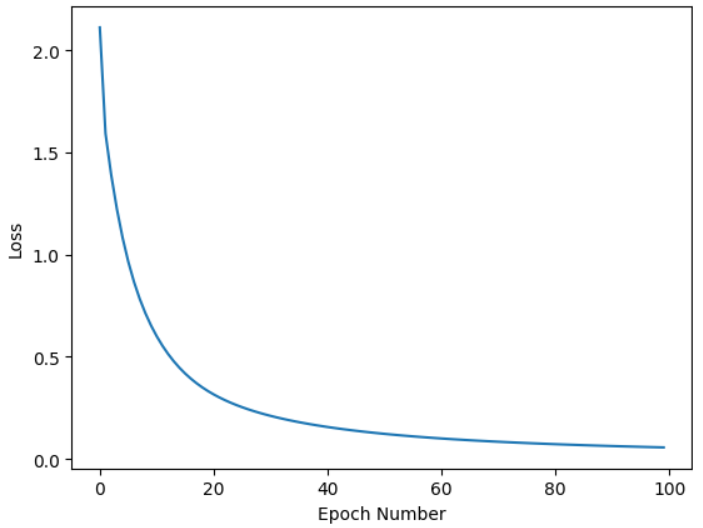
\includegraphics[width=0.6\textwidth]{figures/loss_graph.png} 
    \caption{Training Loss}
    \label{fig:loss_graph}
\end{figure}

\subsubsection{Confusion Matrix}
The confusion matrix provides a detailed breakdown of the model's performance by categorizing predictions into four categories: True Positives (TP), True Negatives (TN), False Positives (FP), and False Negatives (FN). The model is exhibiting high accuracy in classifying the data. It is effectively distinguishing between the two classes with minimal misclassifications. as seen in figure 2 with heat map confusion matrix.

\begin{figure}[H]
    \centering
    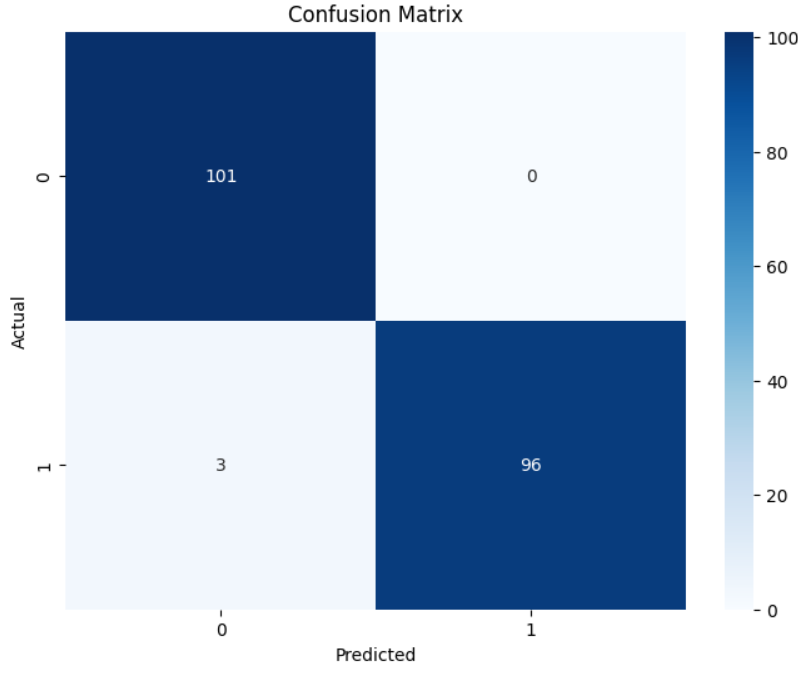
\includegraphics[width=0.75\textwidth]{figures/confusion_matrix.png} 
    \caption{Confusion Matrix}
    \label{fig:confusion_matrix}
\end{figure}

\subsubsection{Classification Report}
We used sklearn library in order to show classification report including: accuracy, precision, recall, and f1.

\textbf{Accuracy}
\begin{equation*}
Accuracy = \frac{TN + TP}{TN + TP + FN + FP}
\end{equation*}
Represents the proportion of correctly classified samples out of the total number of samples in the test set.

\textbf{Precision}
\begin{align*}
    \text{Precision} &= \frac{\text{True Positives}}{\text{True Positives} + \text{False Positives}}
\end{align*}
High precision indicates that the model is reliable in its positive predictions, minimizing the number of false alarms.   

\textbf{Recall}
\begin{align*}\
    \text{Recall} &= \frac{\text{True Positives}}{\text{True Positives} + \text{False Negatives}}
\end{align*}
Recall, also known as sensitivity, measures the model's ability to identify all actual positive instances. High recall ensures that the model effectively captures all relevant instances, minimizing the number of missed detections.

\textbf{F1-Score}

\begin{equation*}
    F1-score = 2 \times \frac{Precision \times Recall}{Precision + Recall}
\end{equation*}
The F1-score is calculated as the harmonic mean of precision and recall. It is a single metric that combines them both.
An F1-score of 1 indicates perfect precision and recall.
A lower F1-score indicates an imbalance between precision and recall. \\ \\
* support - number of samples \\
* macro avg - The average of the metrics (precision, recall, f1-score) calculated for each class, giving equal weight to each class. \\
* weighted avg -  The weighted average of the metrics, where each class is weighted according to its support (number of samples).

\begin{table}[H]
    \centering
    \begin{tabular}{|c|c|c|c|c|}
        \hline
         & precision & recall & f1-score & support \\ \hline
        0 digit sign & 0.97 & 1.00 & 0.99 & 101 \\ \hline
        5 digit sign & 1.00 & 0.97 & 0.98 & 99  \\ \hline
        accuracy &  &  & 0.98 & 200 \\ \hline
        macro avg & 0.99 & 0.98 & 0.98 & 200 \\ \hline
        weighted avg & 0.99 & 0.98 & 0.98 & 200 \\ \hline
    \end{tabular}
    \caption{Model Classification Report}
    \label{tab:classification_report}
\end{table}

The model demonstrates high accuracy (0.98) in classifying sign language digits, with both precision and recall exceeding 0.97 for both classes (0 and 5). This indicates strong performance in accurately identifying and classifying hand gestures representing these digits

\section{Discussion}
Overall, this project provided valuable insights into the application of deep learning for image classification in the context of sign language recognition. We successfully demonstrated the feasibility of utilizing a feed-forward neural network for binary classification of sign language digits (0 and 5). The model achieved high accuracy (0.98) with excellent precision and recall for both classes, indicating strong performance in distinguishing between the two hand gestures.    \\


\underline{Key Findings:} \\
\textbf{Strong Performance} - Employing a simple neural network architecture with a single hidden layer achieved good results, suggesting the potential of deep learning for this task. \\

\underline{Limitations and Considerations:}

\textbf{Dataset Expansion:} Utilize a dataset encompassing all ten sign language digits (0-9) to enhance the model's generalizability and applicability to real-world scenarios.

\textbf{Hyperparameter Tuning:} Further optimize the model through hyperparameter tuning. Experiment with different learning rates, number of neurons in the hidden layer, and other parameters to potentially improve accuracy.

\textbf{Advanced Architectures:} Implement and evaluate more advanced deep learning architectures like CNNs, specifically designed for image classification tasks. These architectures excel at extracting spatial features from images, potentially leading to significant performance gains. \\


\underline{Conclusion} \\
This project has demonstrated the promise of deep learning for basic sign language digit recognition. The achieved accuracy and insights gained provide a valuable foundation for further exploration and development in this area. By addressing the limitations identified, exploring future directions, and considering potential applications, this research can significantly contribute to advancements in deep learning technologies.

\section{Code}
\href{https://colab.research.google.com/drive/17l2Hzcw9iYNcaJ6eD4uKhlNWUl5fsWA1?usp=sharing}{Link to notebook}

\nocite{*} 

Good luck!!
\bibliographystyle{plain}
\bibliography{references.bib}


\end{document}
